\subsection{Target Costing \hfill IP}
    \begin{scriptsize}
        \begin{center}
            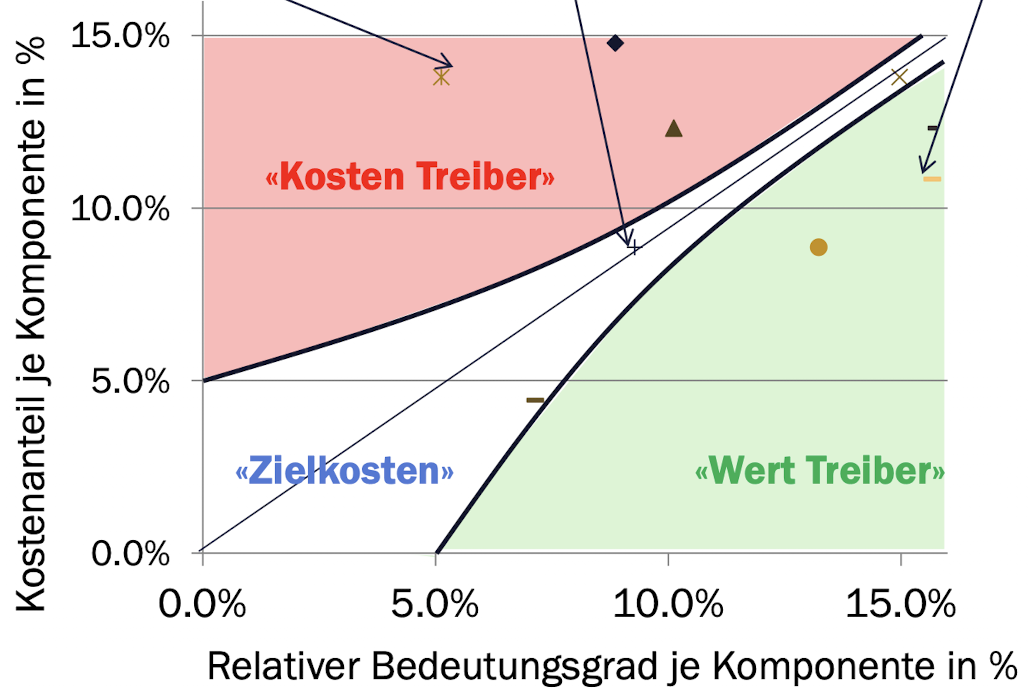
\includegraphics[width = 0.6\linewidth]{MAEIP_Zielkostenmatrix}
        \end{center}
        \begin{itemize}
            \item \textbf{Herkömmlich:} Was wird ein Produkt kosten?
            \item \textbf{Target Costing:} Was darf ein Produkt kosten?
            \item Produkt wird in einzelne Funktionen zerlegt und vom Kunden bewertet
            \item \textbf{Nutzanteil NA:} Anteil der Komponente an Funktionserfüllung multipliziert mit relativer Bedeutung der Funktion
            \item \textbf{Bedeutungsgrad BG:} Summe der Teilgewichte der Komponente pro Funktion
        \end{itemize}
        \vspace{-2mm}
        \mathbox{
            \text{Zielkostenindex} = \frac{BG_{\text{Komponente}}}{\text{Kostenanteil}_{\text{Komponente}}}
        }
    \end{scriptsize}